\section{The Abstract Syntax Tree}
\label{AST}
The AST is the virtuel image of a compiled source code. When the scanner has scanned the input successfully and created a list of tokens, the parser, as described in section \ref{sec:parser}, creates a syntax tree. The AST for the following source code example is represented in figure \ref{fig:astexample}.

\begin{source}{Source code example.}{}
Main (  )
{	
	new Team teamAliens("Aliens", "#FF0000");
	new Agent agentAlice("Alice", 5);
	
	teamAliens.add(agentAlice);	
}
\end{source} 

\begin{figure}[H]
\begin{center}
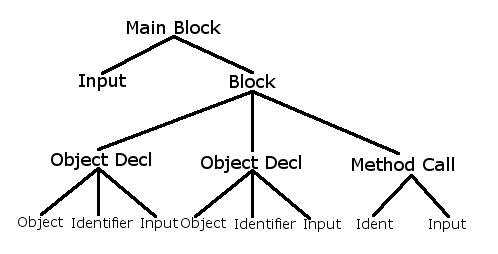
\includegraphics[scale=0.8]{Images/ASTexample.png}
\end{center}
\caption{Example of the AST compiled from the source code above.}
\label{fig:astexample}
\end{figure}

The AST can be printed by a pretty printer\footnote{A method for printing ASTs.} to give a better overview of the compiled source code. In the MASSIVE compiler, the pretty printer prints all completed parses in the windows console. The MASSIVE pretty printer indents whenever a new branch is added. The source code above will be printed as seen in figure \ref{fig:astmasexample}.

\begin{figure}[H]
\begin{center}
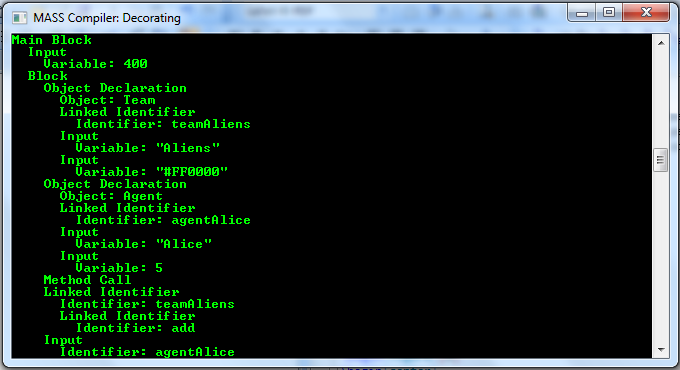
\includegraphics[scale=0.7]{Images/ASTMASexample.png}
\end{center}
\caption{Example of the AST compiled with the MASSIVE compiler.}
\label{fig:astmasexample}
\end{figure}